\chapter{Introducere}

%\chapter*{Introducere}
\label{intro}

\par Conform raportului oficial al Organizației Mondiale a Sănătății \cite{who2019}, aproximativ 2,2 miliarde de oameni trăiesc cu o formă de deficiență de vedere, dintre care cel puțin 1 miliard au o deficiență care ar fi putut fi prevenită sau care nu a fost încă tratată. Impactul funcțional este cel mai sever în rândul celor 43,3 milioane de persoane care suferă de orbire totală și al celor 295 de milioane cu deficiențe moderate până la severe (MSVI) \cite{vleg2021}. Din perspectivă clinică, nevoia de asistență pentru deplasare devine universală odată ce acuitatea vizuală scade sub pragul de $3/60$.

În ceea ce privește mecanismele de sprijin, deși utilizarea câinilor-ghid este considerată în literatura de reabilitare drept reperul pentru fluiditatea mișcării, accesul global rămâne extrem de scăzut. Datele furnizate de International Guide Dog Federation \cite{igdf2023} relevă existența a doar aproximativ 30.000 de câini activi la nivel mondial, ceea ce înseamnă că mai puțin de 0,1\% din populația care ar avea nevoie clinică de un astfel de sprijin beneficiază efectiv de el. Această disparitate este accentuată de barierele economice, costul de antrenament al unui singur exemplar fiind estimat între 40.000\$ și 60.000\$ \cite{cost2018}. În acest context, majoritatea persoanelor cu deficiențe de vedere rămân dependente fie de bastonul alb (utilizat de aproximativ 33,8\% din populația vizată), fie de asistența umană directă \cite{nature2021}.

O evoluție tehnologică recentă, cu un impact semnificativ asupra pieței dispozitivelor portabile (\textit{wearable technology}), este reprezentată de ascensiunea ochelarilor inteligenți (\textit{Smart Glasses}) \ref{fig:figures/aria-gen-2-specs.png}. Această categorie de dispozitive a fost popularizată recent prin parteneriate strategice, precum cel dintre Meta și Ray-Ban \cite{metarayban}, care au integrat senzori optici performanți în accesorii de uz cotidian. Din punct de vedere tehnic, prezența camerei video pe aceste dispozitive permite captarea și procesarea fluxului vizual în timp real, oferind astfel o platformă potențială pentru sisteme de asistență computațională.

\begin{figure}[htbp]
    \centering
    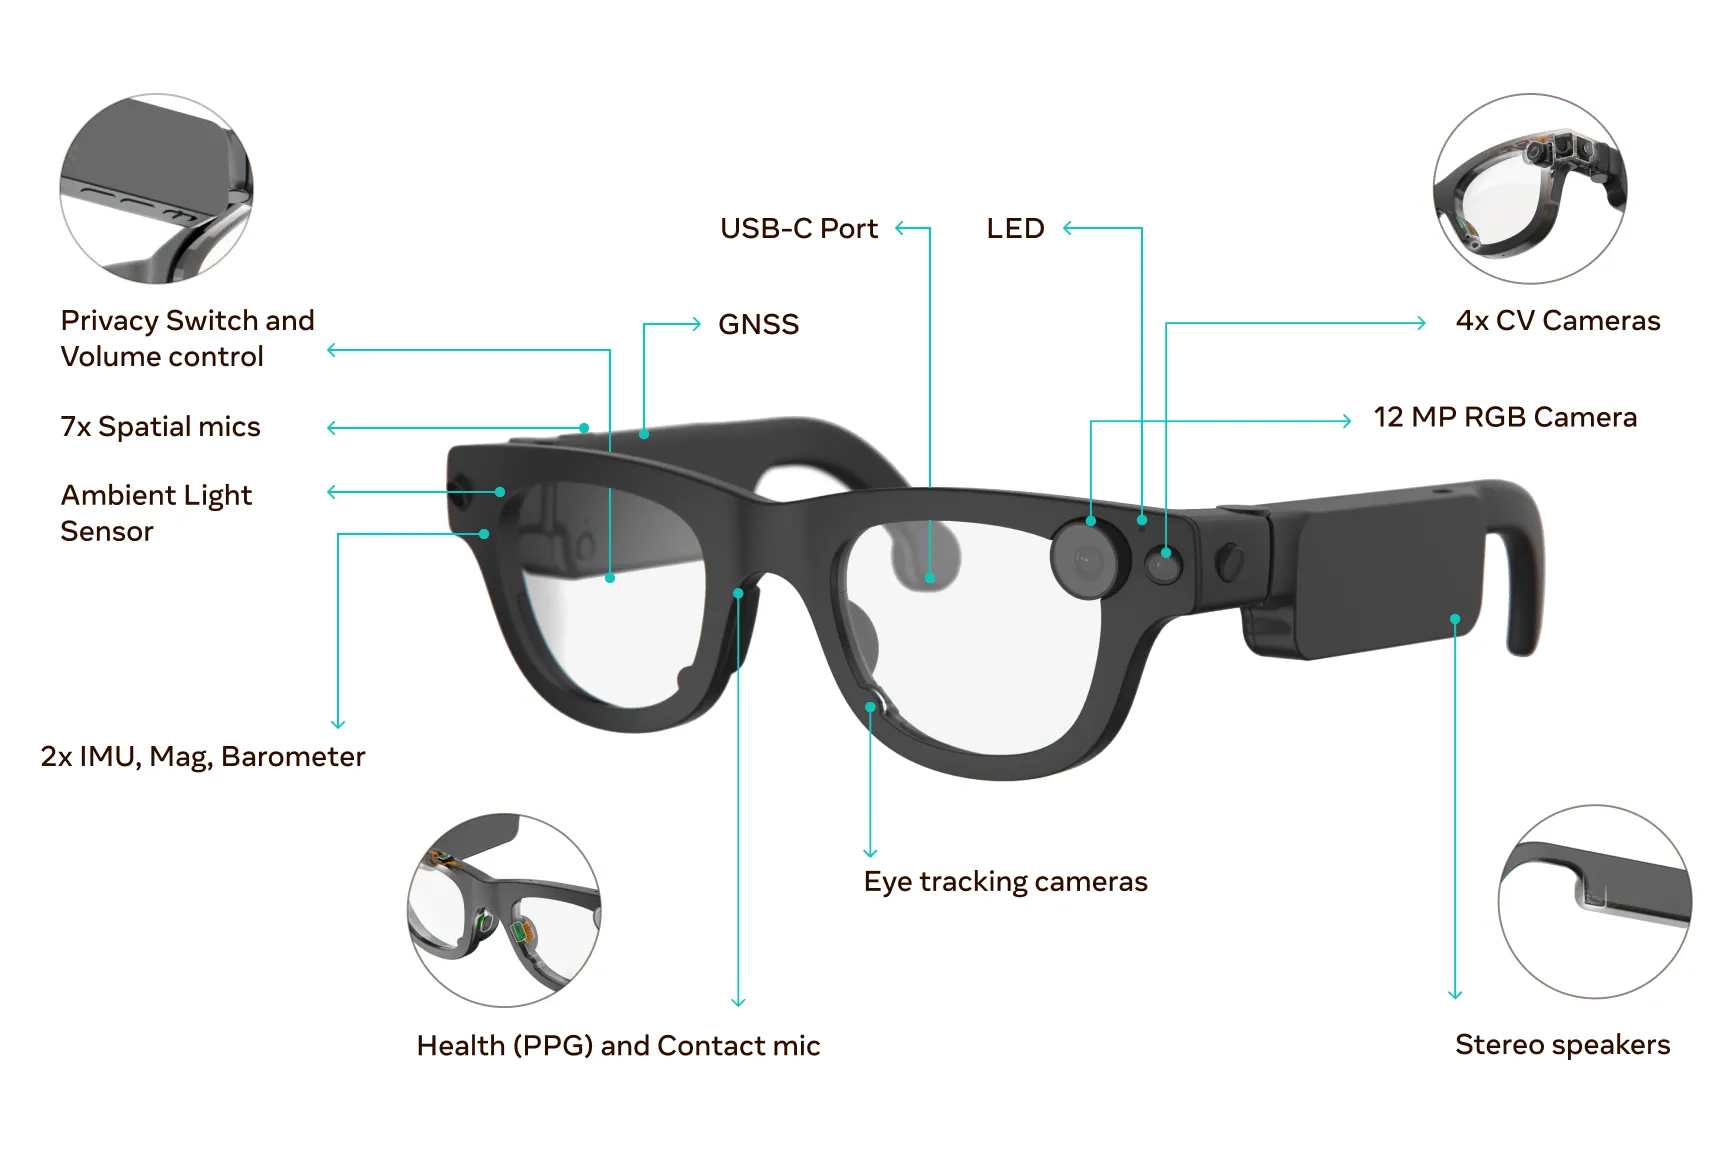
\includegraphics[width=0.7\linewidth]{figures/aria-gen-2-specs.png}
    \caption{Exemplu de dispozitiv de tip Smart Glasses, Aria Gen 2. Sursă: \href{https://roadtovrlive-5ea0.kxcdn.com/wp-content/uploads/2025/06/aria-gen2.jpg}{Road to VR}}
    \label{fig:figures/aria-gen-2-specs.png}
\end{figure}

Cu toate acestea, deși ochelarii Ray-Ban Meta oferă funcționalități AI impresionante, precum recunoașterea obiectelor și a scenelor din jur, traducerea în timp real, identificarea textului din mediul înconjurător și asistentul vocal integrat bazat pe Meta AI \cite{metarayban}, această tehnologie puternică rămâne limitată în privința utilității pentru persoanele cu deficiențe de vedere. Cea mai utilizată aplicație dedicată acestui segment al populației este Be My Eyes \cite{bemyeyes}, o platformă care conectează utilizatorii nevăzători cu voluntari ce le oferă asistență vizuală în timp real prin intermediul camerei telefonului. Limitarea fundamentală a acestei soluții constă în dependența de disponibilitatea voluntarilor umani, ceea ce o face inadecvată pentru scenarii de navigație autonomă continuă sau pentru situații în care intervenția imediată este esențială.

În acest context considerăm că hardware-ul existent și inovațiile recente din domeniul inteligenței artificiale ar permite dezvoltarea de aplicații care să permită persoanelor cu deficiente de vedere, o independență mult mai ridicată care nu se bazează pe ghizi canini.

Motivată de nevoia critică de independență a persoanelor cu deficiențe severe de vedere și valorificând accesibilitatea actuală a tehnologiei de tip \textit{Smart Glasses}, prezenta lucrare propune dezvoltarea unui sistem compact și eficient din punct de vedere al costurilor. Obiectivul principal al sistemului este de a sprijini utilizatorul în detectarea și evitarea obstacolelor, facilitând astfel o mobilitate mai sigură și mai autonomă.

Lucrarea de față abordează tocmai acest gol: investigarea și implementarea unui sistem de detecție și evitare a obstacolelor destinat persoanelor cu deficiențe de vedere, construit pe o platformă accesibilă din punct de vedere financiar, în special Raspberry Pi \cite{raspberrypi5}. Procesul de dezvoltare a debutat pe o platformă de tip x86 echipată cu o unitate de procesare grafică dedicată, urmând ca soluția să fie ulterior portată pe platforma țintă. Această strategie de dezvoltare în două etape a condus la diferențe măsurabile de performanță între cele două configurații hardware, diferențe datorate în principal capacității de procesare superioare oferite de GPU-ul dedicat. Din acest motiv, pe parcursul lucrării ambele platforme sunt analizate comparativ, iar rezultatele obținute pe fiecare sunt prezentate în paralel. Deși platforma țintă rămâne Raspberry Pi, rezultatele superioare înregistrate pe platforma de dezvoltare sunt incluse ca referință pentru a ilustra potențialul maxim al algoritmilor propuși.

Structura lucrării este organizată după cum urmează: Capitolul~\ref{chap:ch2} trece în revistă literatura de specialitate ce a stat la baza creionării sistemului descris în lucrare. Ulterior, în Capitolul~\ref{chap:ch3} este prezentată metodologia de dezvoltare și sunt analizate dificultățile tehnice întâmpinate. Capitolul~\ref{chap:ch4} descrie arhitectura aplicației propuse. În Capitolul~\ref{chap:ch5} sunt prezentate și discutate performanțele obținute pe cele două platforme hardware. În final, Capitolul~\ref{conclusions} sintetizează concluziile lucrării și propune direcții viitoare de cercetare.

\section{Utilizarea instrumentelor IA generative}
\label{sec:ai_usage}

În timpul elaborării acestei lucrări, autorul a folosit Claude Opus 4.8 pentru a găsi erori în codul sursă, a refactoriza fișiere de cod, și pentru a reformula porțiuni din prezenta lucrare. După utilizarea acestui instrument/serviciu, autorul a revizuit și editat conținutul generat și își asumă întreaga responsabilitate pentru conținutul lucrării.
